\begin{figure}[t]
  \centering
  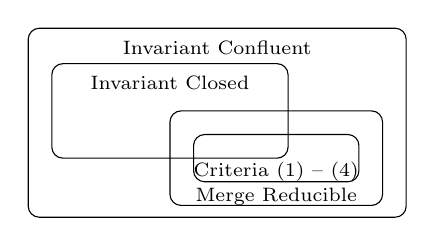
\begin{tikzpicture}[scale=0.3]
    \draw[rounded corners] (0, 0) rectangle (16, 8);
    \draw[rounded corners] (1, 2.5) rectangle (11, 6.5);
    \draw[rounded corners] (6, 0.5) rectangle (15, 4.5);
    \draw[rounded corners] (7, 1.5) rectangle ++(7, 2);
    \node[inner sep=0pt, anchor=north] at (8, 7.5) {\scriptsize Invariant Confluent};
    \node[inner sep=0pt, anchor=north] at (6, 6) {\scriptsize Invariant Closed};
    \node[inner sep=0pt, anchor=south] at (10.5, 1.5) {\scriptsize Criteria (1) -- (4)};
    \node[inner sep=0pt, anchor=south] at (10.5, 0.5) {\scriptsize Merge Reducible};
  \end{tikzpicture}
  \caption{%
    The relationship between \invariantclosure{}, \mergereducibility{},
    criteria (1) -- (4) from \thmref{LatticeProperty}, and
    \invariantconfluence{}.
  }\figlabel{IclosureVsReducible}
\end{figure}
